\documentclass{standalone}
\usepackage{tikz}
\usepackage{tikz-network}
\usepackage{subcaption}
\usepackage{graphicx}
% \usetikzlibrary{graphs, graphdrawing, positioning, quotes}
\usepackage{color}
\definecolor{lightblue}{RGB}{158,202,225}

\begin{document}

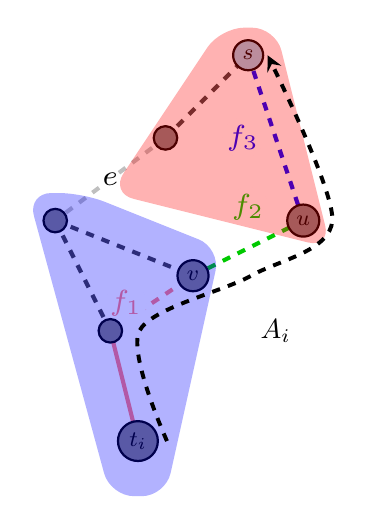
\begin{tikzpicture}[scale=0.7]
		\coordinate (s) at (2,2);
		\coordinate (e_upper) at (0.5,0.5);
		\coordinate (e_lower) at (-1.5,-1);
		\coordinate (t_i) at (0,-5);
		\coordinate (t_1) at (-2,-5);
		\coordinate (t_iup) at (-0.5,-3);
		\coordinate (u) at (3,-1);
		\coordinate (v) at (1,-2);
		\node[draw,circle,fill=lightblue,thick,inner sep=2pt,minimum size=5pt] (CircleNode) at (s)  {\footnotesize $s$};
		\node[draw,circle,fill=gray,thick,inner sep=2pt,minimum size=5pt] (CircleNode) at (t_i)  {\footnotesize $t_i$};
		\node[draw,circle,fill=gray,thick,inner sep=3pt,minimum size=5pt] (CircleNode) at (e_upper){};
		\node[draw,circle,fill=gray,thick,inner sep=3pt,minimum size=5pt] (CircleNode) at (e_lower){};
		\node[draw,circle,fill=gray,thick,inner sep=3pt,minimum size=5pt] (CircleNode) at (t_iup){};
		\node[draw,circle,fill=gray,thick,inner sep=2pt,minimum size=5pt] (CircleNode) at (u){\footnotesize $u$};
		\node[draw,circle,fill=gray,thick,inner sep=2pt,minimum size=5pt] (CircleNode) at (v){\footnotesize $v$};
	
		\draw [ draw=none,rounded corners = 3mm,fill= blue,fill opacity=0.3]([shift={(-0.5,0.5)}]e_lower)--([shift={(0.5,0.5)}]e_lower)--([shift={(0.5,0.5)}]v)--([shift={(0.5,-1)}]t_i)--([shift={(-0.5,-1)}]t_i)--cycle;
	
		\draw [ draw=none,rounded corners = 3mm,fill=red,fill opacity=0.3]([shift={(0.5,0.5)}]s)--([shift={(0.5,-0.5)}]u)--([shift={(-1,-1)}]e_upper)--([shift={(-0.5,0.5)}]s)--cycle;  
	
		\Edge[style={dashed},label=$e$,fontcolor=black,fontscale =1.5,color=gray!50](e_upper)(e_lower)
		\Edge[style={dashed}](e_lower)(t_iup)
		\Edge[style={dashed}](e_lower)(v)
		\Edge[style={dashed}](e_upper)(s)
		\Edge[color=red!50](t_i)(t_iup)
		\Edge[style={dashed},color=red!50,label=$f_1$,position={above=1.5mm,left=0.1mm},fontscale=1.5](t_iup)(v)
		\Edge[style={dashed},RGB,color={0,201,0},label=$f_2$,position={above=2mm},fontscale=1.5](v)(u)
		\Edge[style={dashed},color=blue,label=$f_3$,position={above=2mm,left=1mm},fontscale=1.5](s)(u)
		\draw[line width=0.5mm,dashed,-stealth] plot[smooth] coordinates {([xshift=15pt]t_i)([xshift=15pt]t_iup)([xshift=30pt]v) ([xshift=15pt]u) ([xshift=10pt]s)};
		\node at (2.5,-3){$A_i$};
	\end{tikzpicture}
\end{document}